\section{Fakes}

\subsection{Hvad er Fakes?}
En Fake er en falsk version af en klasses dependancy.

\subsection{Hvorfor bruge Fakes?}
Når vi ønsker at isolere vore UUT fra det system det normalt fungerer i, for at teste det i isolation.

\subsection{Hvordan bruges Fakes?}

\begin{itemize}
	\item Identificer dependencies.
	\item Insert interfaces for dem
	\item Inject dependencies ind i UUT. \todo{eksempel}
\end{itemize}

\subsection{Statebaserede tests og Interactionbaserede tests}
Der findes to typer af Unit tests:

\begin{itemize}
	\item State-Based - Hvor vi tester om UUT er i det forventede state efter behandling. Fakes til denne type af test er en \textbf{STUB}.
	\item Interaction-Based - Hvor vi tester om UUT har den ønskede adfærd efter behandling. Her kigges der på UUT's adfærd med dens dependencies. Fakes til denne type af test er en \textbf{MOCK}.
\end{itemize}

\subsection{Stubs}
Stubbe eksisterer kun for at give UUT de dependancies den behøver for at fungere.
Hvis en klasse Calculator er afhængig af en klasse der kan lave beregninger, kan der laves en stub af denne klasse, der blot returnerer en fastlagt værdi. 

Procedure for stubbe:
\begin{itemize}
	\item Arrange - Opsætning af UUT og dens dependancies.
	\item Act - Stimuler UUT'en. Få den til at gøre det vi ønsker.
	\item Assert - Assert på om vi får det ønskede resultat, altså om UUT's state er den ønskede.
\end{itemize}

Bemærk at Assert sker på UUT og \textit{ikke} på selve stubben. En stub kan derfor ikke forårsage en fejlet test.

\begin{figure}
	\centering
	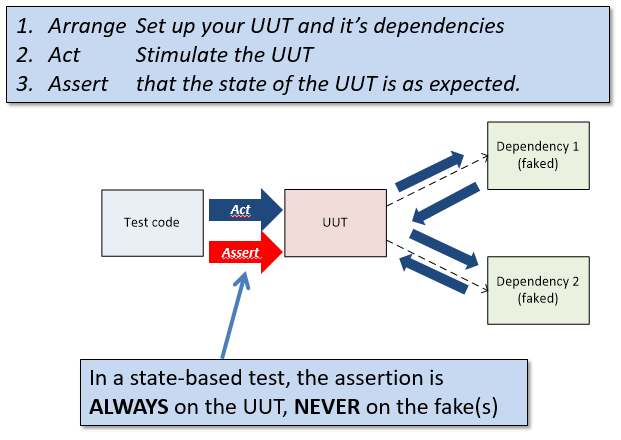
\includegraphics[width=0.7\linewidth]{figs/stubTest.PNG}
	\caption{Unit testing med stubbe.}
	\label{fig:stubTest}
\end{figure}

Vi ønsker at lave en state baseret test på klassen A. Klassen A har en afhængighed Class B.

\begin{figure}[H]
	\centering
	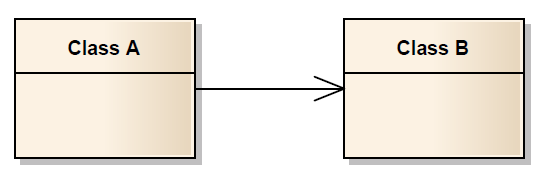
\includegraphics[width=0.7\linewidth]{figs/stubNoInterface.PNG}
	\caption{Afhængighed - DIP ikke opfyldt.}
	\label{fig:stubNoInterface}
\end{figure}

Brugen af et interface vil her give mening. Vi påfører DIP of får da:

\begin{figure}[H]
	\centering
	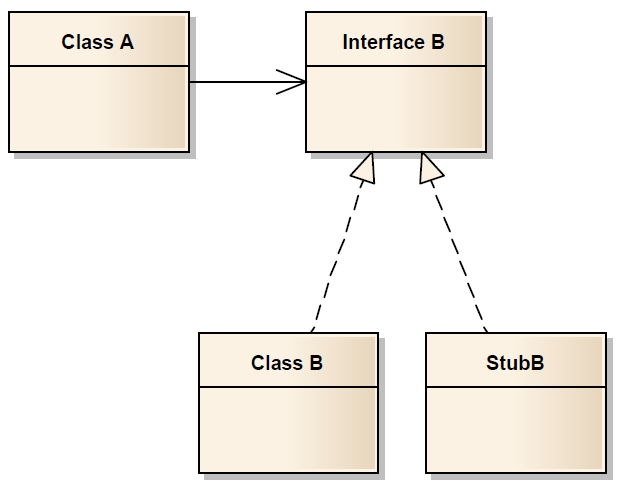
\includegraphics[width=0.7\linewidth]{figs/stubInterface.PNG}
	\caption{}
	\label{fig:stubInterface}
\end{figure}

Her laves en en stub af interfacet B, hvorefter man kan bruge stubben til at teste UUT i et kontrolleret miljø.

\subsubsection{Constructor injection}
Stubbe handler om at teste stadier. Det kan da være en fordel at anvende constructor injection.

\todo{eksempel på ctor injection ifbm. stubbe}

\todo{Persketivér til ATM opgaven}

\subsection{Mocks}
Mocks relaterer sig til adfærdsbaserede tests, og ikke ændrer sig selv, men derimod andre. Der assertes derfor på en anden klasse end den selv.

\begin{figure}[H]
\centering
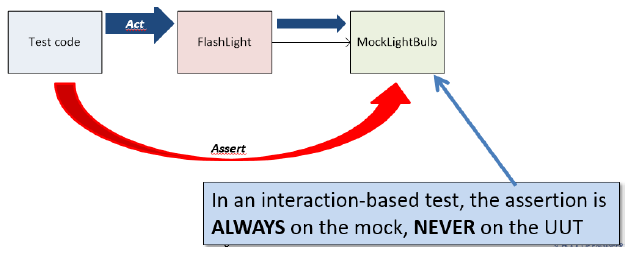
\includegraphics[width=0.7\linewidth]{figs/mockTest.PNG}
\caption{Unit testing med mock}
\label{fig:mockTest}
\end{figure}

Da der med Mocks, testes om UUT har gjort de forventede operationer på dens dependencies, bliver mock-klassen nødt til at recorde om operationen er sket.

Procedure for stubbe:
\begin{itemize}
	\item Arrange - Opsætning af UUT og dens dependancies.
	\item Act - Stimuler UUT'en. Få den til at gøre det vi ønsker.
	\item Assert - Assert på om mock klassen blev interageret med korrekt af UUT.
\end{itemize}

Det er i modsætning til stubbe, muligt for en mock klasse at få en test til at fejle.

Da en mock skal indeholde nogle recordings er en mock typisk mere tidskrævende at skrive, og samtidig sværere at genbruge.

\todo{Indsæt eksempel på en mock}